% What we want vs what the example controller typically gets on a mini rig:
% motor demand (top) and speed (bottom) while the rider pedals and then
% stops. Illustrative curves, used in the worksheet and the slides.
\documentclass[11pt, border=2pt]{standalone}
\usepackage{pgfplots}
\usepgfplotslibrary{groupplots}
\pgfplotsset{compat=1.18}

\begin{document}
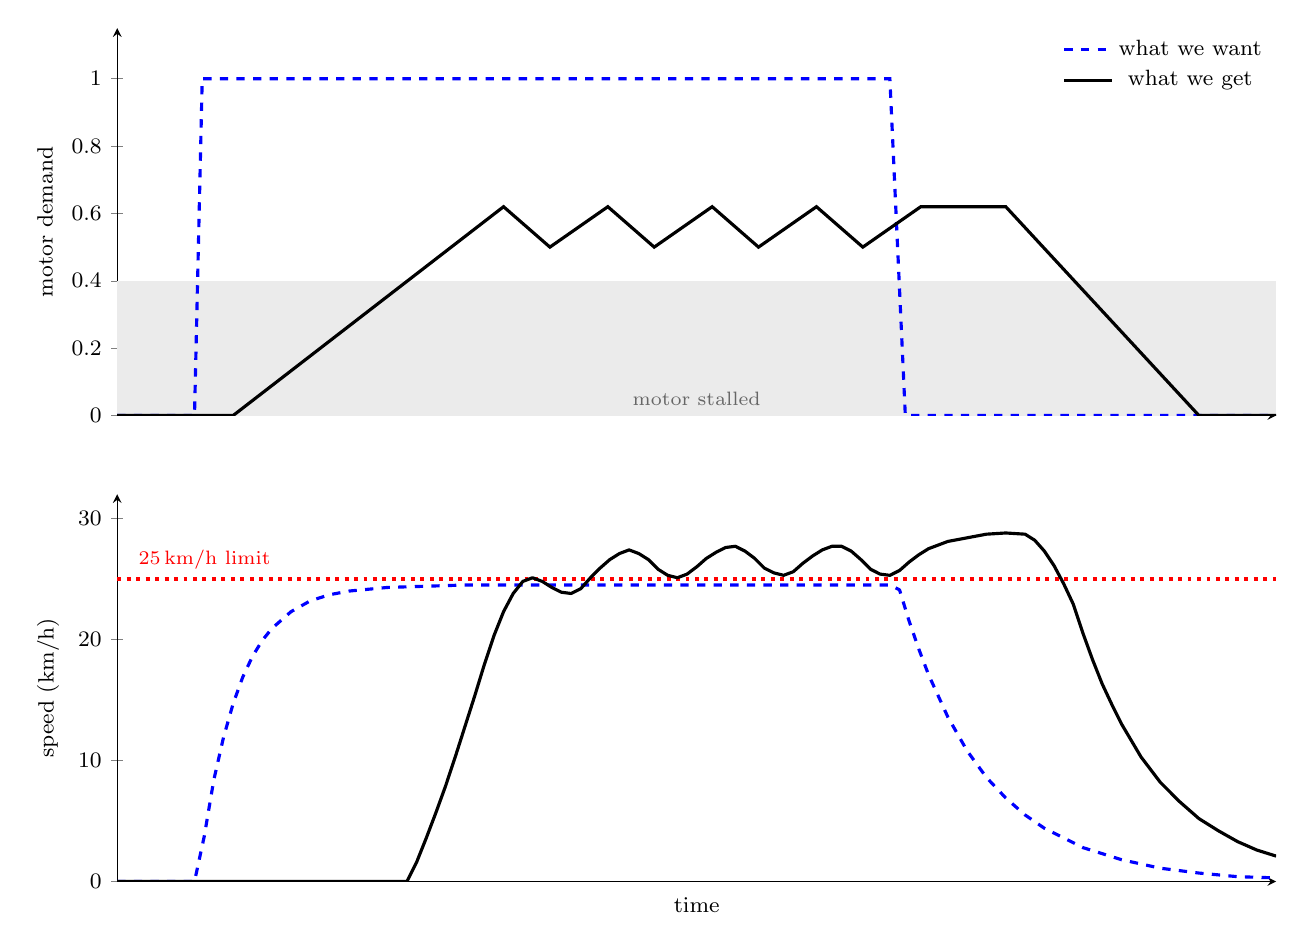
\begin{tikzpicture}
    \begin{groupplot}[
        group style={group size=1 by 2, vertical sep=1cm},
        width=16.3cm, height=6.5cm,
        xmin=0, xmax=30, axis lines=left, xtick=\empty,
        tick label style={font=\footnotesize},
        label style={font=\footnotesize},
        legend style={font=\footnotesize, draw=none, fill=none,
            at={(1, 1)}, anchor=north east},
    ]
        \nextgroupplot[ymin=0, ymax=1.15, ylabel={motor demand},
            ytick={0, .2, .4, .6, .8, 1}]
            % below about 0.4 the motor doesn't turn at all
            \fill[black!8] (axis cs:0, 0) rectangle (axis cs:30, .4);
            \node[font=\scriptsize, anchor=south, text=black!60]
                at (axis cs:15, 0) {motor stalled};
            % full help for as long as the rider pedals
            \addplot[line width=.4mm, dashed, blue] coordinates {
                (0,0) (2,0) (2.2,1) (20,1) (20.4,0) (30,0)};
            \addplot[line width=.4mm, black] coordinates {
                (0,0) (3,0) (10,.62) (11.2,.5) (12.7,.62) (13.9,.5)
                (15.4,.62) (16.6,.5) (18.1,.62) (19.3,.5) (20.8,.62)
                (23,.62) (28,0) (30,0)};
            \legend{what we want, what we get}
        \nextgroupplot[ymin=0, ymax=32, ylabel={speed (km/h)},
            xlabel={time}]
            \draw[red, line width=.5mm, dotted]
                (axis cs:0, 25) -- (axis cs:30, 25);
            \node[font=\scriptsize, anchor=south west, text=red]
                at (axis cs:.3, 25) {25\,km/h limit};
            % both speed curves come from a simple model of the rig:
            % the speed lags behind a target set by the demand (zero
            % below about 0.4, about 25 km/h at 0.55), faster when
            % speeding up than when coasting down
            \addplot[line width=.4mm, dashed, blue, line join=round]
                coordinates {
                (0,0) (2,0) (2.25,3.7) (2.5,8.4) (2.75,11.9) (3,14.7)
                (3.25,16.9) (3.5,18.6) (3.75,19.9) (4,20.9)
                (4.5,22.3) (5,23.2) (5.5,23.7) (6,24) (7,24.3)
                (8,24.4) (9,24.5) (20,24.5) (20.25,24.1) (20.5,21.5)
                (20.75,19.2) (21,17.1) (21.5,13.6) (22,10.8)
                (22.5,8.6) (23,6.9) (23.5,5.5) (24,4.4) (25,2.8)
                (26,1.8) (27,1.1) (28,0.7) (29,0.4) (30,0.3)};
            \addplot[line width=.4mm, black, line join=round]
                coordinates {
                (0,0) (7.5,0) (7.75,1.6) (8,3.6) (8.25,5.7) (8.5,7.9)
                (8.75,10.3) (9,12.8) (9.25,15.3) (9.5,17.9)
                (9.75,20.3) (10,22.3) (10.25,23.8) (10.5,24.8)
                (10.75,25.1) (11,24.8) (11.25,24.3) (11.5,23.9)
                (11.75,23.8) (12,24.2) (12.25,25.1) (12.5,25.9)
                (12.75,26.6) (13,27.1) (13.25,27.4) (13.5,27.1)
                (13.75,26.6) (14,25.8) (14.25,25.3) (14.5,25.1)
                (14.75,25.4) (15,26) (15.25,26.7) (15.5,27.2)
                (15.75,27.6) (16,27.7) (16.25,27.3) (16.5,26.7)
                (16.75,25.9) (17,25.5) (17.25,25.3) (17.5,25.6)
                (17.75,26.3) (18,26.9) (18.25,27.4) (18.5,27.7)
                (18.75,27.7) (19,27.3) (19.25,26.6) (19.5,25.8)
                (19.75,25.4) (20,25.3) (20.25,25.7) (20.5,26.4)
                (20.75,27) (21,27.5) (21.5,28.1) (22,28.4)
                (22.5,28.7) (23,28.8) (23.5,28.7) (23.75,28.2)
                (24,27.3) (24.25,26.1) (24.5,24.6) (24.75,22.9)
                (25,20.5) (25.25,18.3) (25.5,16.3) (25.75,14.6)
                (26,13) (26.5,10.3) (27,8.2) (27.5,6.6) (28,5.2)
                (28.5,4.2) (29,3.3) (29.5,2.6) (30,2.1)};
    \end{groupplot}
\end{tikzpicture}
\end{document}
